\documentclass[pageno]{jpaper}

%replace XXX with the submission number you are given from the ASPLOS submission site.
\newcommand{\asplossubmissionnumber}{XXX}

\usepackage[normalem]{ulem}

\begin{document}

\title{
Tensor-intact Compilation for Ubiquitous Machine Learning Computers}

\date{}
\maketitle

\thispagestyle{empty}

\begin{abstract}

Machine learning computers (MLCs) equipped with tensor functional units for improved efficiency have attracted increasing attentions recently. To fully take advantage of MLCs, there is a huge demand for programming infrastructures to gain extremely high performance across highly diverse architectures. Although existing programming tools are aware of the importance of the \emph{tensor} for easing the programming burden (e.g., programming directly with tensor semantic), they neglect to use tensor semantic for low-level hardware-specific optimization, and thus lose potential optimization opportunities in tensor-oriented MLCs.

In this paper, we propose the Tensor-Intact Compilation (TIC) that preserves the tensor semantic for generalized and aggressive hardware-specific compilation optimization across ubiquitous MLCs. The key intuition is that \emph{by integrating abstract hardware information of MLCs into the tensor optimization can lead to a larger optimization space for automatic searching}, compared to traditional approaches that decouples high-level tensor optimizations (e.g., layout transform) and low-level scalar optimizations (e.g., loop tiling). Concretely, TIC is implemented by the proposed Tensor Intermediate Representation (TIR) on the Tensor Abstract Machine (TAM). TAM is the foundation of TIC by abstracting the characteristics of tensor processing in a broad range of MLCs. Based on TAM, various hardware-specific tensor-level optimizations on TIR are proposed and can be generally deployed across ubiquitous MLCs. Experimental results show that TIC outperforms state-of-art programming infrastructures on 3 commodity ML computers including GPU with Tensor Cores, TPU, and MLU.
\end{abstract}

\section{Introduction}

Machine learning (ML) algorithms have been widely used in a broad range of application fields, such as computer vision~\cite{liu2016ssd}, speech signal processing~\cite{amodei2016deep}, machine translation~\cite{bahdanau2014neural}, and robotics~\cite{redmon2015real}. To improve the processing efficiency of ML algorithms, Machine Learning Computers (MLCs) equipped with tensor functional units have emerged to deliver significantly better performance and energy efficiency than general-purpose architectures. Typical commodity MLCs include NVIDIA's GPU with Tensor Cores specially designed for accelerating matrix and convolutional operations~\cite{markidis2018nvidia}, Google's Tensor Processing Units (TPU) for tensor operations~\cite{jouppi2017datacenter}, and Cambricon's Machine Learning Unit (MLU) for general machine learning operations~\cite{cambrion2016url}.


The programming infrastructure is crucial to effectively take advantage of various MLCs. However, the key challenge is to achieve high performance across highly diverse architectures. Figure~\ref{fig:challenge} shows that $4$ well-known programming infrastructures (i.e., TensorFlow~\cite{abadi2016tensorflow}, PyTorch~\cite{paszke2017automatic}, TVM~\cite{chen2018tvm}, and MLIR~\cite{Lattner2020MLIR}) perform significantly different on not only the same GPU platform but also $3$ different platforms (i.e., GPU, Tensor Cores, and TPU), and no one can dominate the others. This challenge is mainly caused by non-trivial exploitation of highly parallel computation units and intricate memory hierarchy of MLCs. Though ML compilers (e.g., XLA~\cite{tensorflow2016xla} and TVM) have emerged as a promising technique for automatically generating optimized code for different backend platforms, it still requires a great amount of expert efforts for achieving high performance, especially when porting to a new MLC. For example, TVM requires the programmers manually implementing dedicated schedules with schedule primitives (e.g., split, fuse, reorder, and tensorize), and the manual implemented schedules significantly vary for different ML architectures. 

\begin{figure}[t]

\centering
  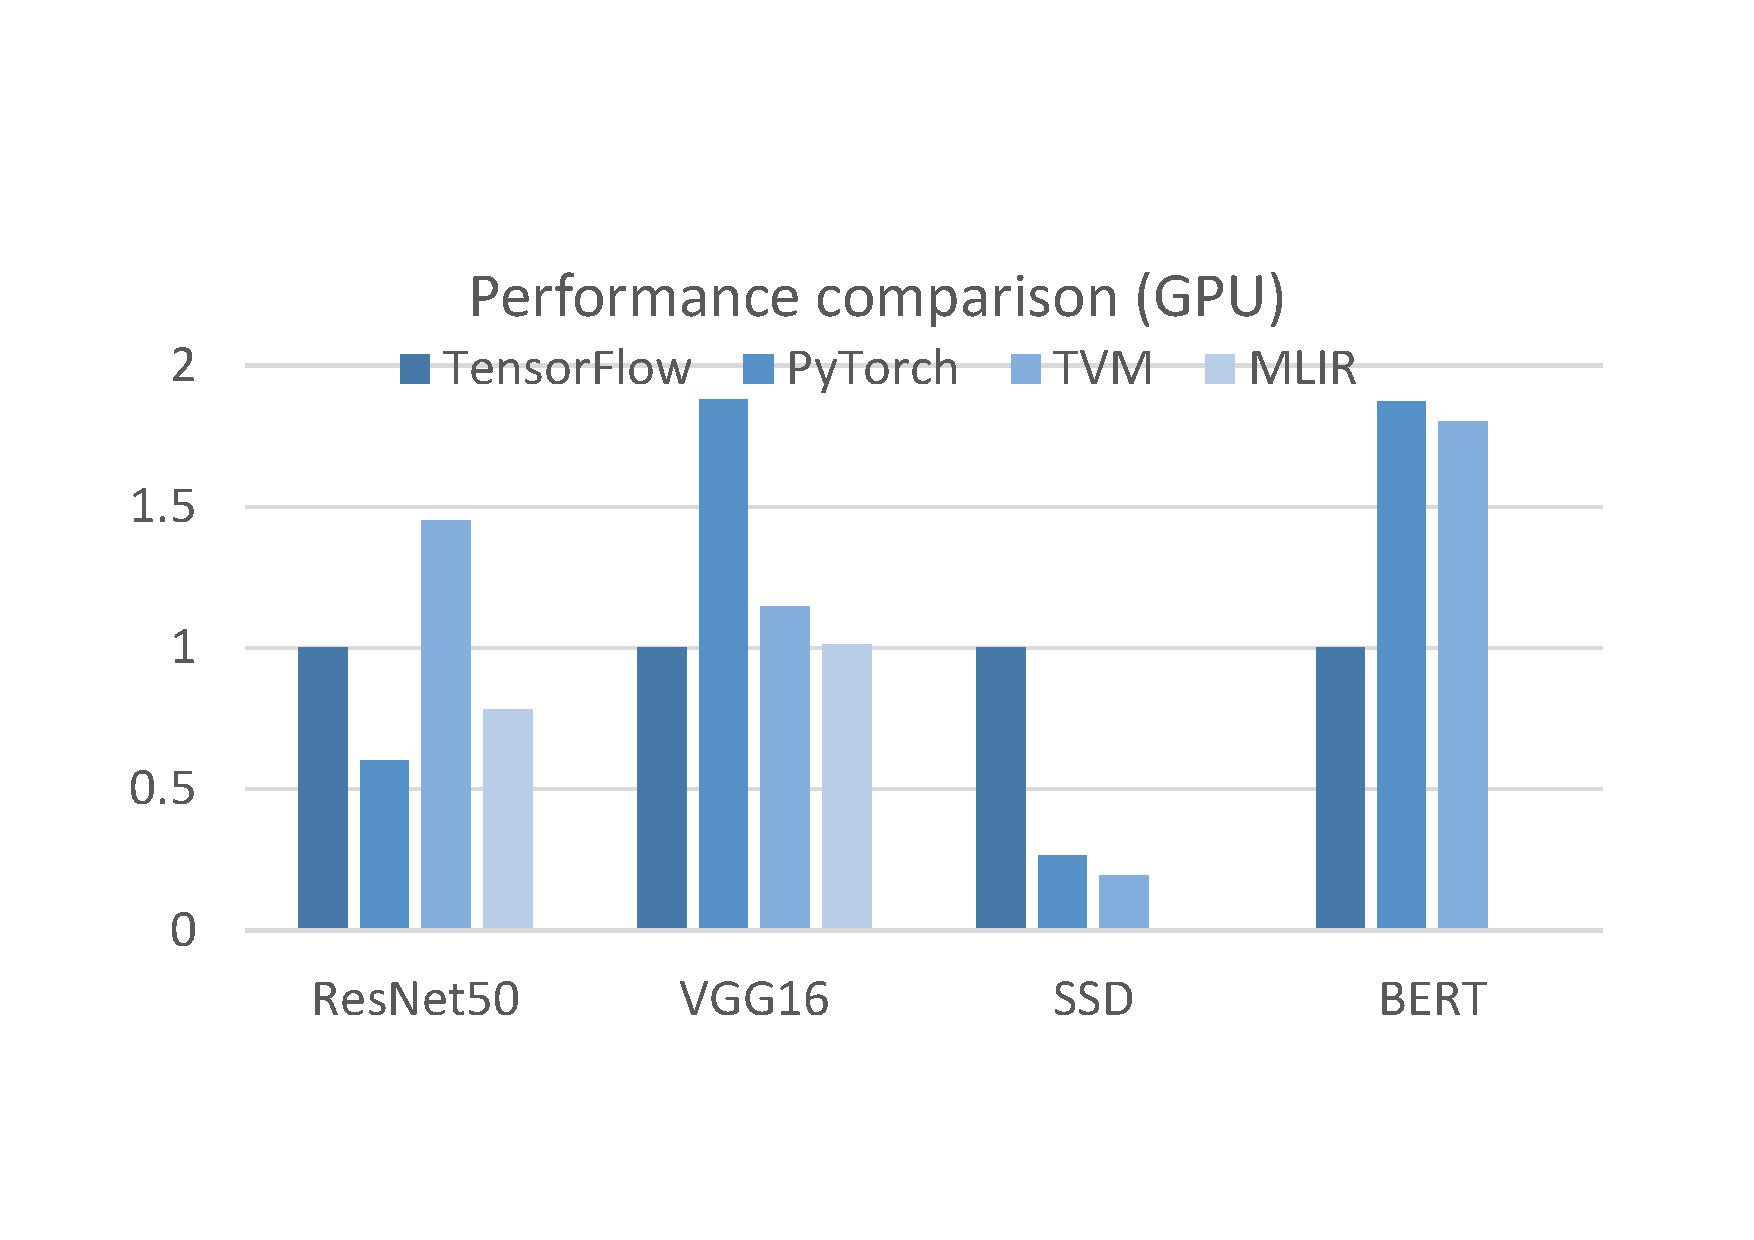
\includegraphics[width=0.44\columnwidth]{figures/intro-perf-gpu.pdf}
  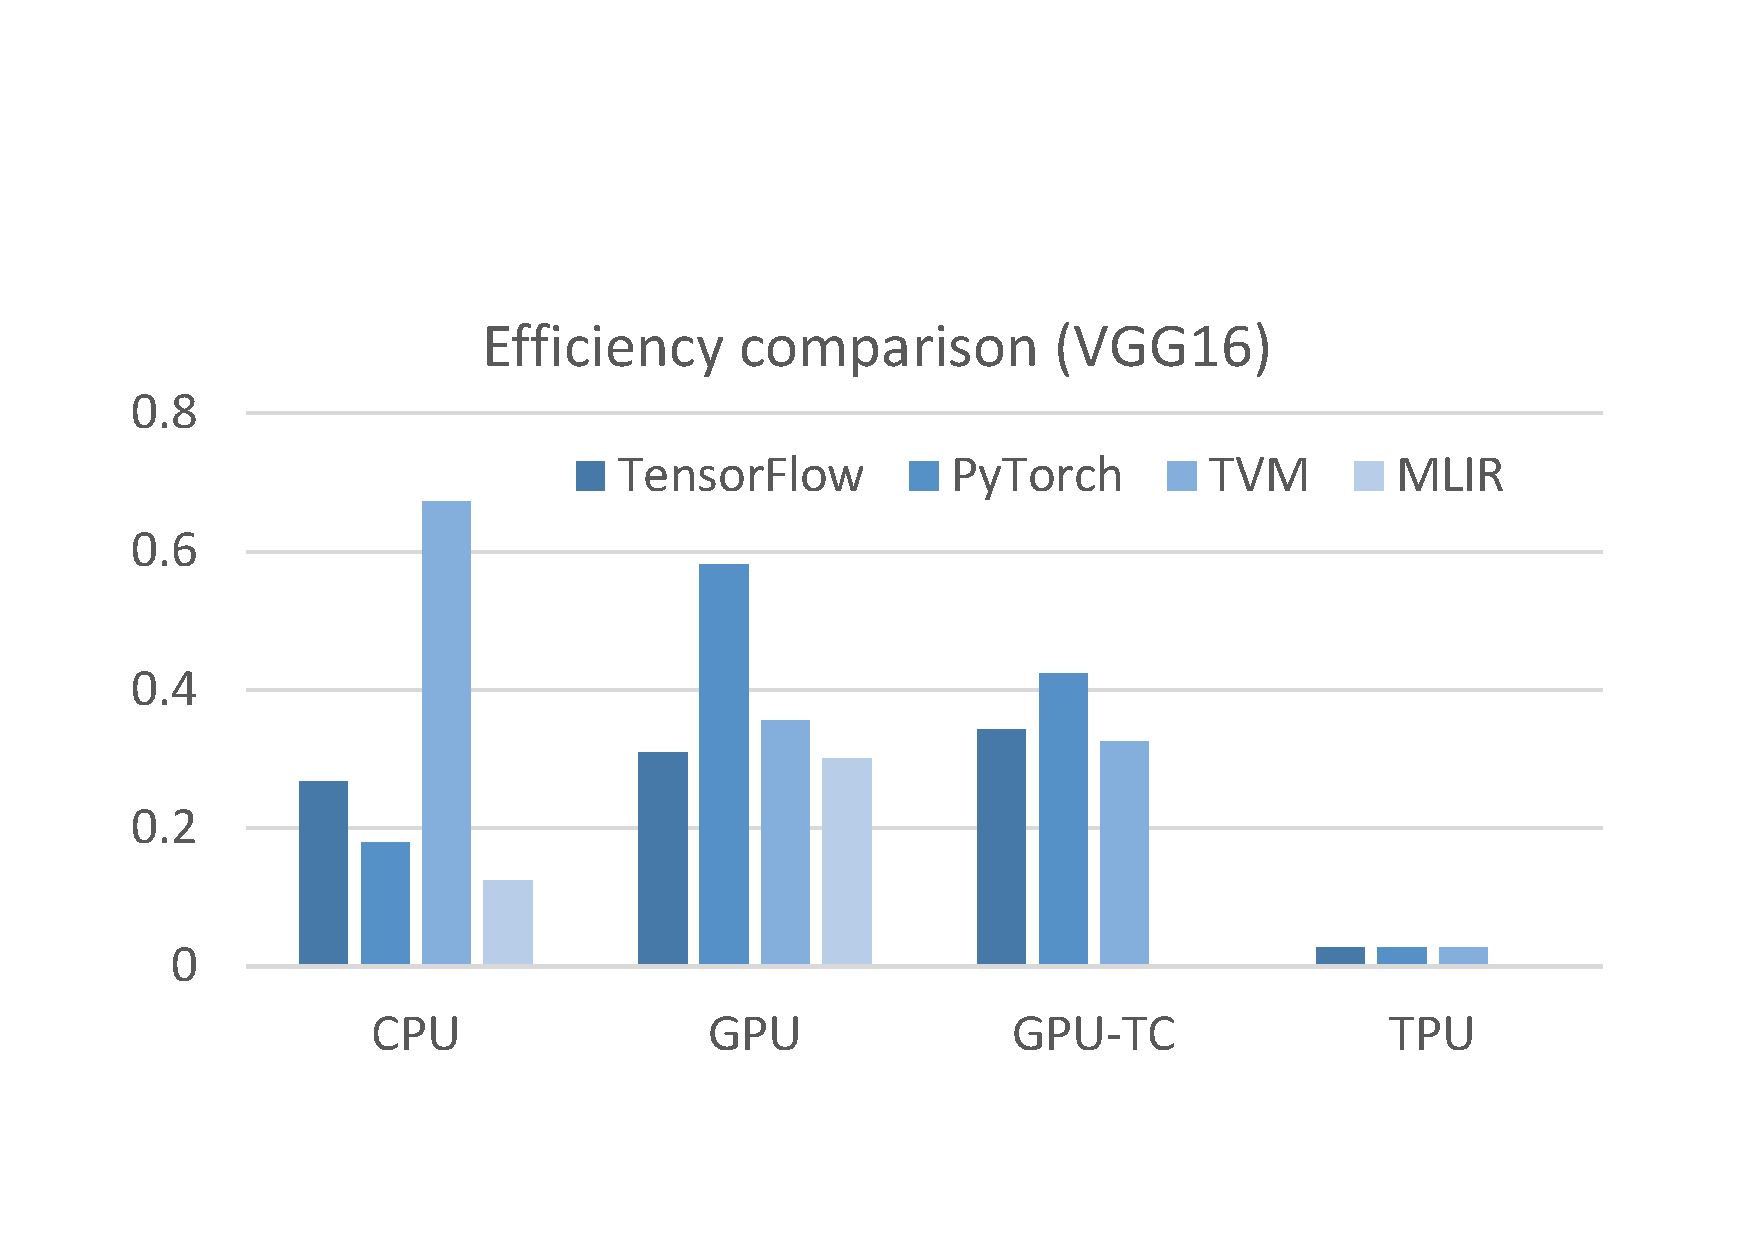
\includegraphics[width=0.44\columnwidth]{figures/intro-eff.pdf}
\caption{\footnotesize The comparison of four programming infrastructures (i.e., TensorFlow, PyTorch, TVM, and MLIR). (a) It is hard to optimize the performance of applications for different programming infrastructures even on the same GPU platform (the performance is normalized to that of TensorFlow). (b) Even for the same application (VGG16~\cite{simonyan2014very}), the efficiency (i.e., hardware utilization) varies significantly across different platforms for evaluated programming infrastructures. Apparently, none of the above programming infrastructures can dominate others for exploiting the computational ability.}
%The key challenges of programming infrastructures for ML computers, which are mainly caused by the huge gap between $M$ ML applications and $N$ hardwares. (b) The \emph{performance} challenge: it is hard to optimize the performance of applications with $4$ different programming infrastructures (i.e., TensorFlow, PyTorch, TVM, and MLIR) even on the same GPU platform (the higher the better). (c) The \emph{productivity} challenge: the programming efforts of applications vary significantly for different infrastructures even on the same GPU platform (the lower the better). (d) The \emph{portability} challenge: for a specific application (i.e., ResNet50), the performance portability is different across $N$ platforms (the higher the better). Apparently, none of the above programming infrastructure can dominate others.}
%given a specific application, it is hard to optimize the performance even on one platform ($1$ vs $1$). (c) The productivity challenge: given $M$ applications, the productivity varies significantly even on one platform ($M$ vs $1$). (d) The portability challenge: given a specific application, it is hard to ensure performance portability across different platforms ($1$ vs $N$).}
\label{fig:challenge}

\end{figure}

The key reason of the inefficiency of existing programming infrastructures (including ML compilers) is that \emph{the critical tensor semantic generated from the high-level programming interfaces is broken during the lowering process for ML accelerators, which directly process tensor semantic as well}. Here we use two motivating examples in TensorFlow and TVM to demonstrate that breaking the tensor semantic during compilation is inefficiency for ML architectures.


%though most of them directly handle tensors instead of scalars, e.g., TensorFlow characterizes the execution as dataflow graphs by carrying \emph{tensors} on the edges. Here we use two motivating examples in TensorFlow and TVM to demonstrate that breaking the tensor semantic during compilation is inefficiency for ML architectures.

\textbf{Framework example (e.g., TensorFlow).} Figure~\ref{fig:intro-tf} shows the overall execution of the \texttt{max\_pool} operation in TensorFlow, where the tensor semantic is broken during the implementation of this operation, i.e., from the high-level TensorFlow API to the low-level CUDA implementation. In the CUDA code, the original \texttt{max\_pool} operation is broken into scalar operations (e.g., conditional comparison) with multiple loops. Thus, for the ML architecture equipped with tensor instructions (e.g., \texttt{VGTM}, Vector-Greater-Than-Merge instruction in~\cite{liu2016cambricon,chen2019instruction}), non-trivial optimization (e.g., notorious auto-parallelization) should be conducted either manually or automatically on the scalar operations to leverage such tensor instructions, which is extremely hard and may result in low performance and huge efforts.

%A potential solution is to extend the low-level language to directly support tensor instructions.

%\begin{figure}[t]
%  \centering
%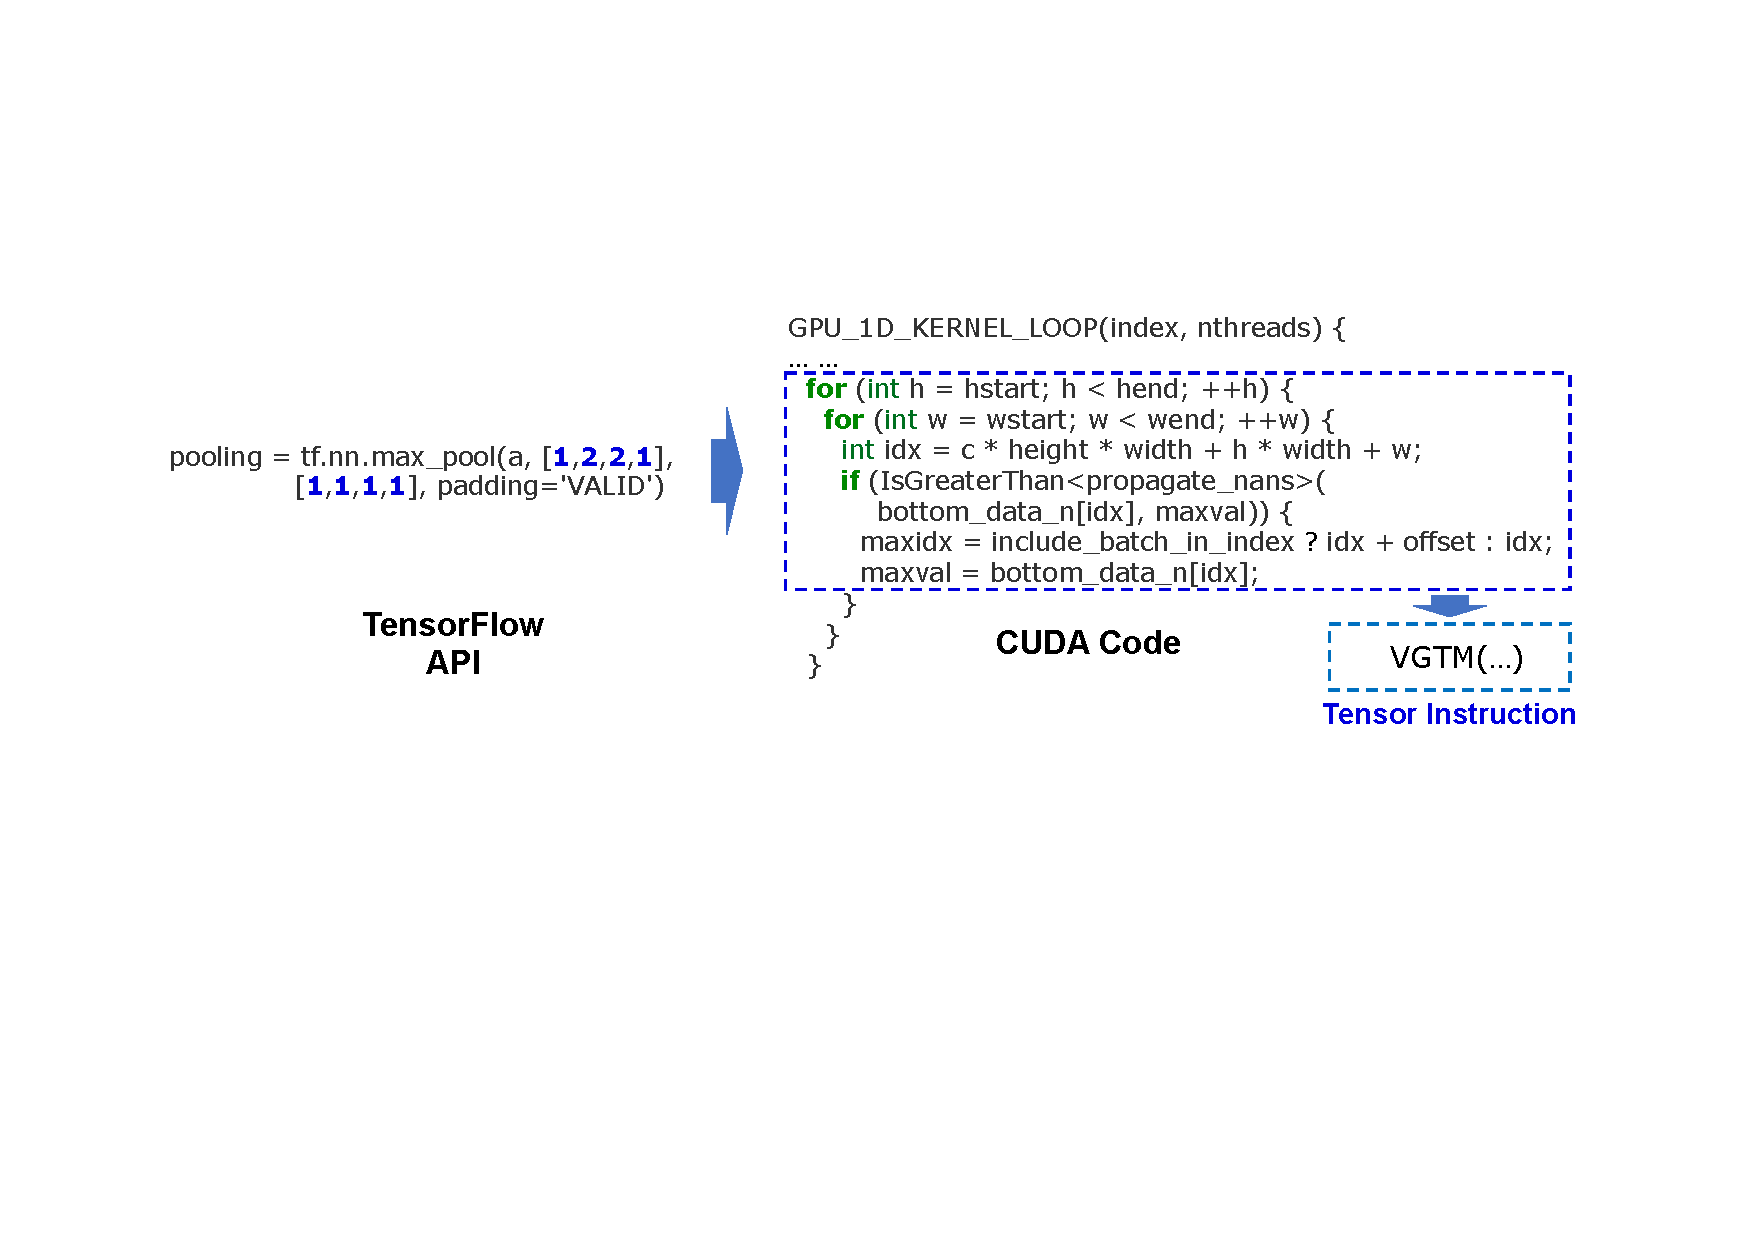
\includegraphics[width=1.0\columnwidth]{figures/intro-tf.pdf}
%\caption{\footnotesize The tensor semantic is broken from the high-level \emph{tensor} API to low-level \emph{scalar} implementation, which makes it extremely hard to exploit the tesnor instructions (e.g., \texttt{VGTM}) of ML hardware from the low-level code.}
%\label{fig:intro-tf}
%\end{figure}

\textbf{ML compiler example (e.g., TVM).} Figure~\ref{fig:intro-tvm} shows the execution of the \texttt{conv} operation in TVM for GPU with Tensor Cores (GPU-TC) and Cambricon-ACC (CACC)~\cite{chen2019instruction}, where the input is Relay's graph IR that directly processes tensors. After converting the Relay IR to the TVM IR, the tensor operation is lowered into multiple loops with scalar multiply and add operations. Then, the TVM IR can be \emph{tensorized} to target platforms with tensor-related primitives, such as \texttt{wmma::mma\_sync} and \texttt{conv} in GPU-TC and CACC, respectively. Apparently, such ``tensor-scalar-tensor" process is relatively tedious and error-prone for either manually or automatically leveraging tensor-related primitives and inflexible for enforcing tensor-level optimizations such as tensor decomposition and tensor pipeline. In addition to low productivity and potential performance loss, the optimization on TVM IR for supporting tensor primitives is not portable across different architectures. For example, \texttt{wmma::mma\_sync} cannot be executed on CACC. %Therefore, it is necessary to provide abstraction of common tensor processing of underlying ML architectures to improve the portability.

%\begin{figure*}
%\centering
%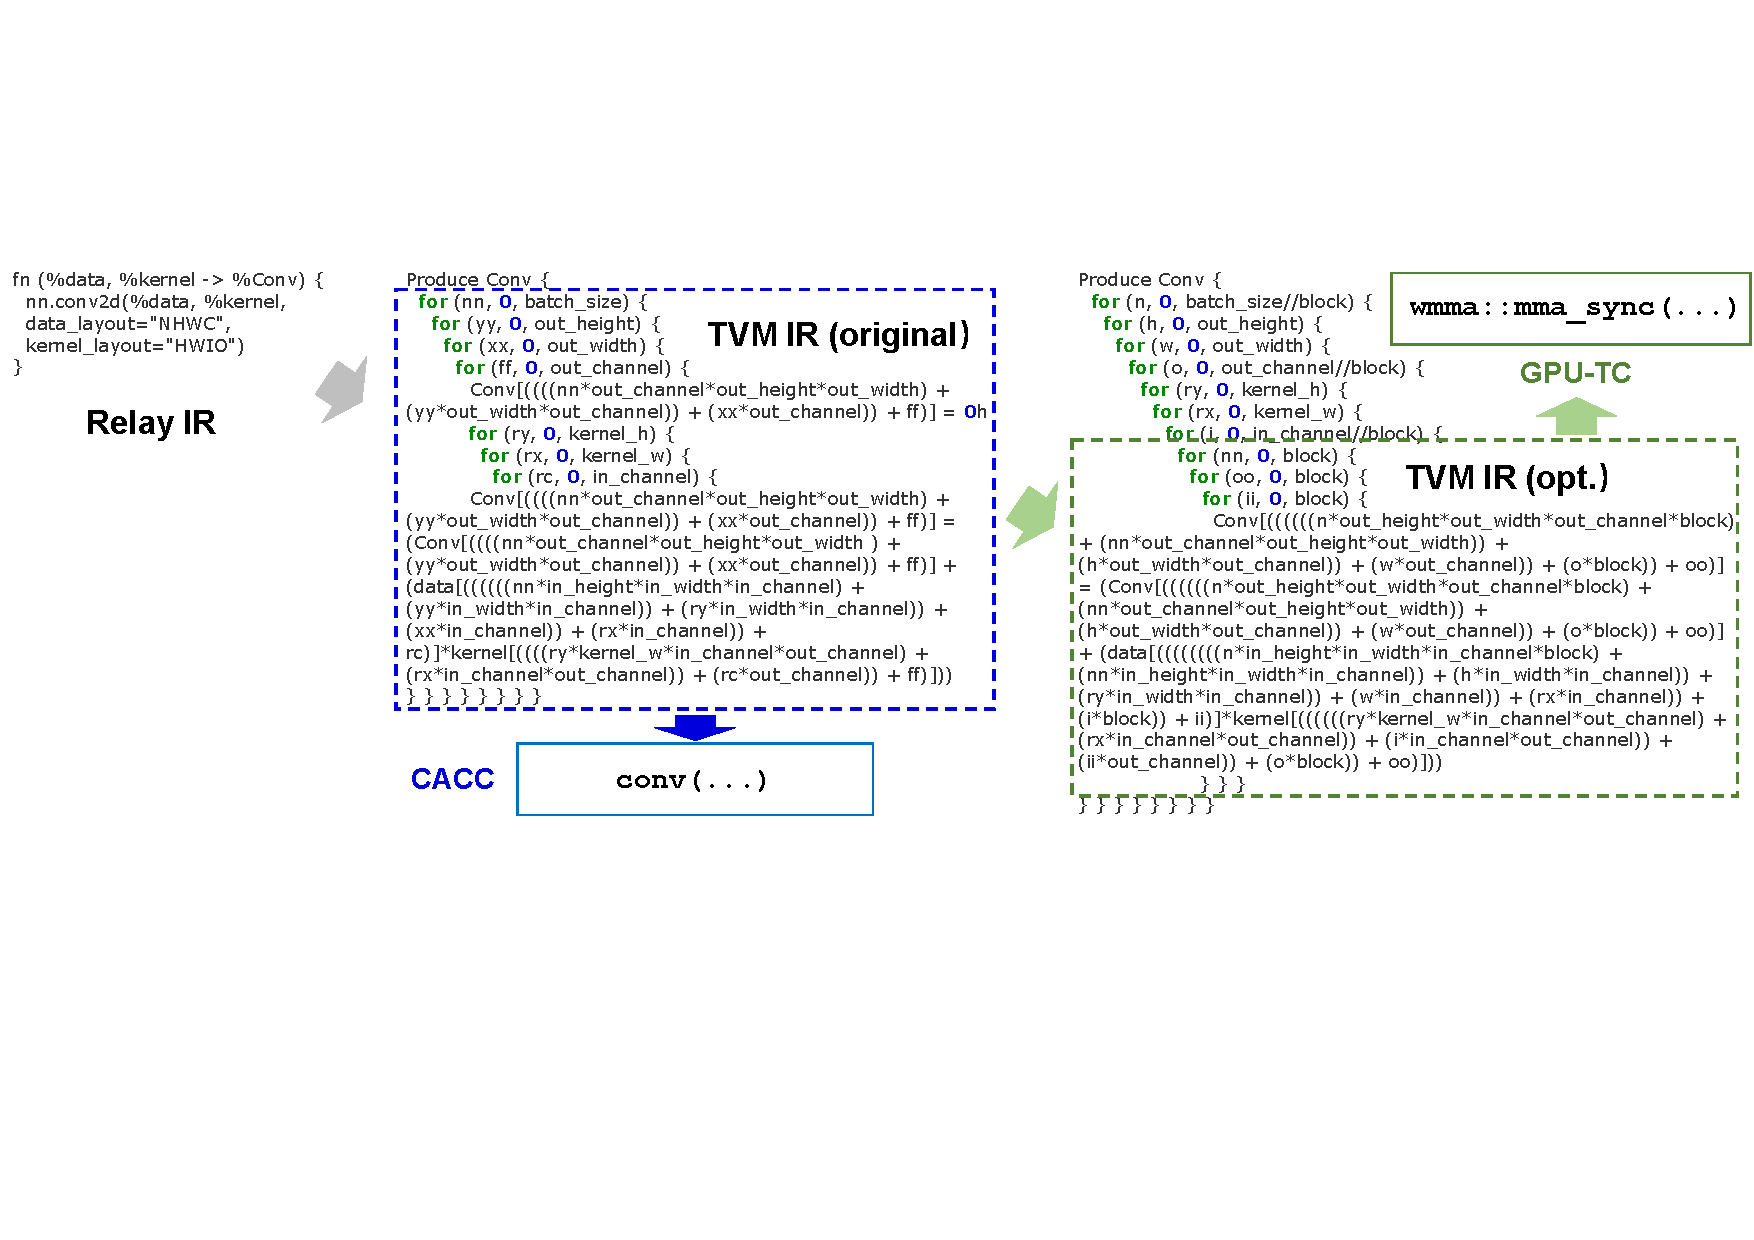
\includegraphics[width=0.9\textwidth]{figures/intro-tvm.pdf}
%\caption{\footnotesize The tensor semantic is broken during the lowering process in TVM for GPU with Tensor Cores (GPU-TC) and Cambricon-ACC (CACC), where the ``tensor-scalar-tensor" process is relatively tedious and may lose potential performance optimization, For GPU-TC, the original IR requires dedicated optimization for using \texttt{wmma:mma\_sync}. For CACC, it is relatively intuitive for using the \texttt{conv} primitive. Also, the direct extension of TVM IR for supporting tensor primitives without abstraction of various ML architectures results in low portability across different platforms.}
%\label{fig:intro-tvm}
%\end{figure*}

\textbf{Our solution.} Based on the above observation, in this paper, we propose the Tensor-Intact Compiling (TIC) infrastructure for ML computers. As shown in Figure~\ref{fig:intro-comp}, the key of TIC is to replace the previous scalar-based low-level IR with tensor-based IR (i.e., Tensor Intermediate Representation, TIR), which can represent tensor primitives and specific memory hierarchy for tensor processing, so that the tensor semantic can be preserved from the input high-level IR (e.g., Relay IR, TensorFlow Graph IR) to tensor-oriented hardware platforms (e.g., GPU-TC, TPU, and CACC). In order to perform tensor-related optimizations, an abstract tensor machine (i.e., Tensor Abstract Machine, TAM) is proposed for concealing the huge variety of ML architectures. Specifically, by raising the level of abstraction of tensor processing in various ML architectures, many common hardware-aware optimizations such as \emph{tensor decomposition} and \emph{tensor alignment} can be conducted at high levels to alleviate the porting burden across different platforms. This is completely different in previous approaches where the tedious manual or semi-automatic tensorization should be performed for each platform. Moreover, in addition to high-level tensor-based IR, we also propose a domain-specific language, Tensor-Aware Language (TAL), with tensor semantic and hardware characteristics (e.g., memory hierarchy and control logic) for manually achieving extremely high performance. To our best knowledge, such a compiling infrastructure preserving tensor sematic across abstract hardware machine, hardware-aware IR, and programming language is the first holistic solution for addressing the performance challenge of various ML computers.

%\begin{figure}[t]
%\centering
%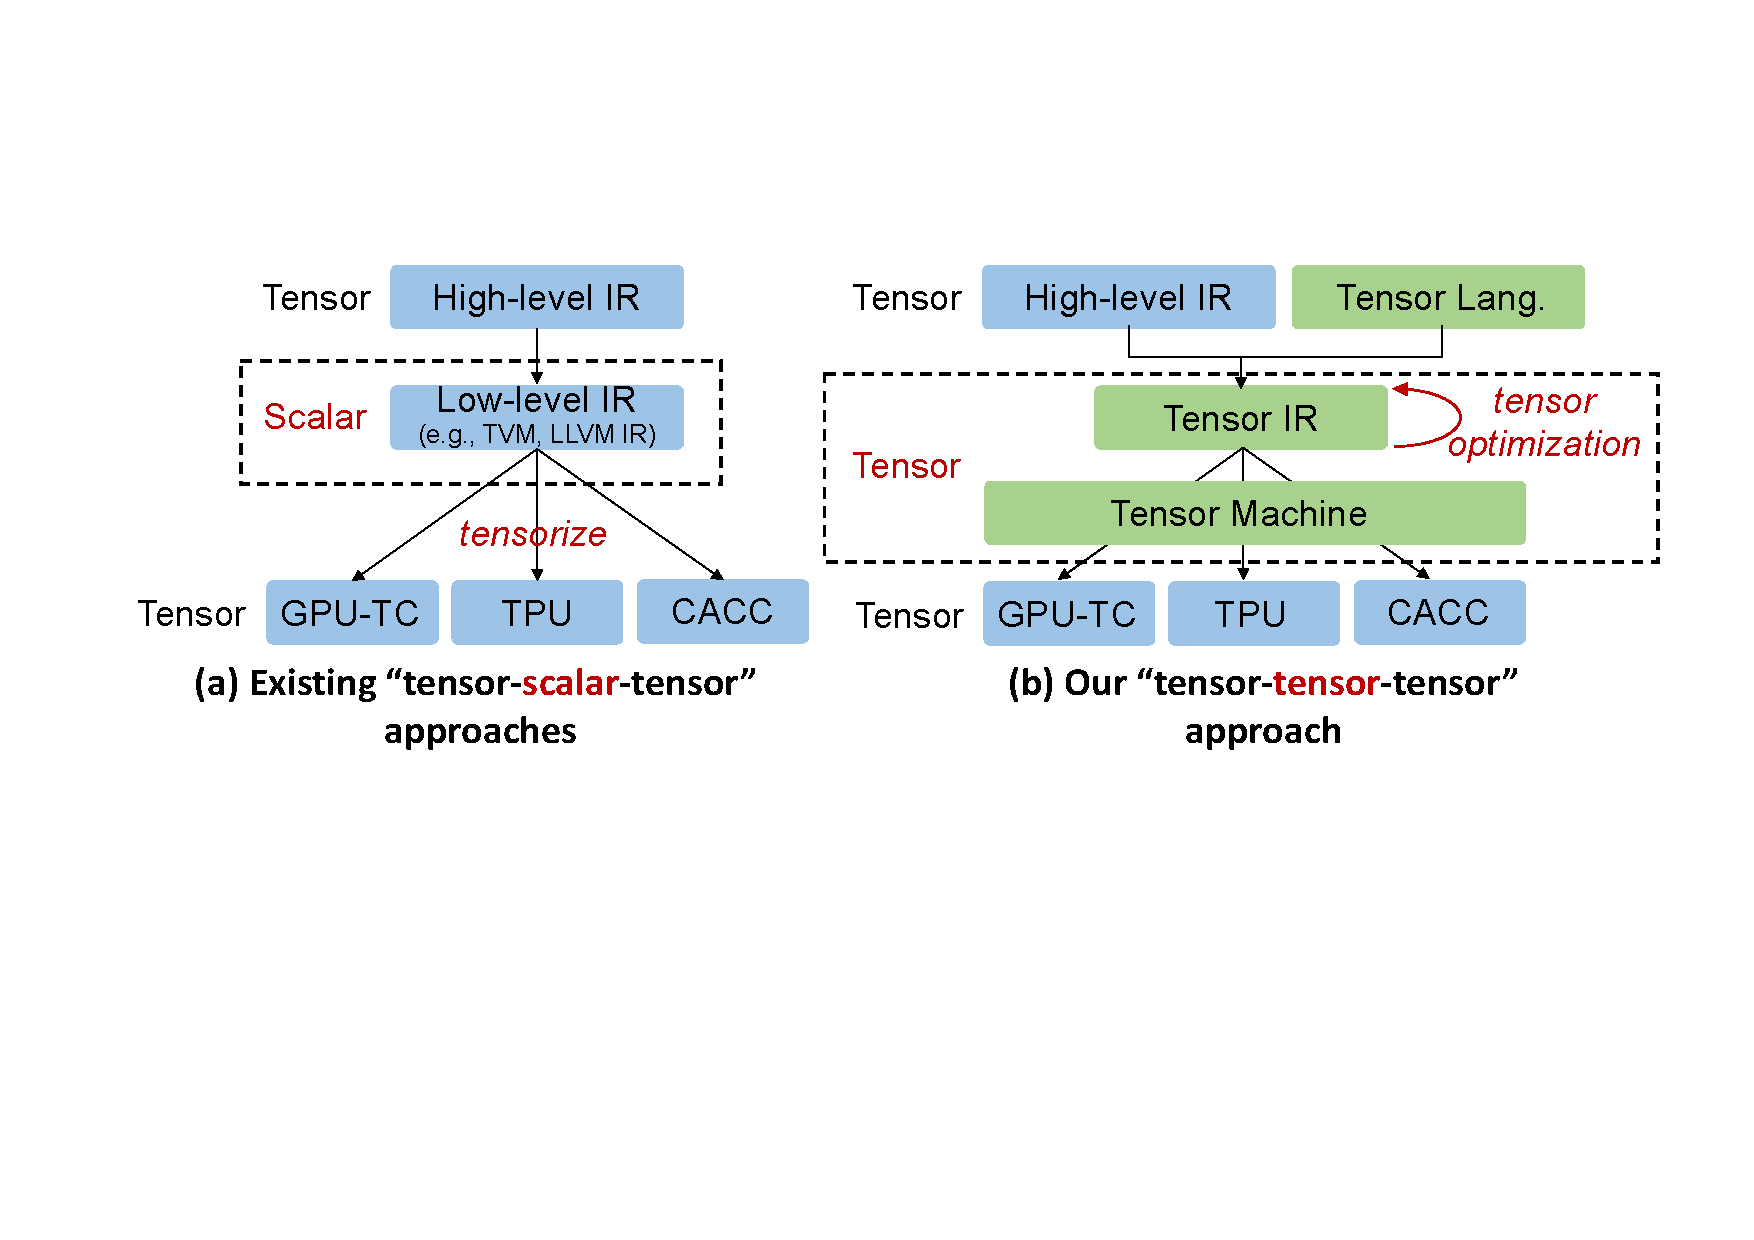
\includegraphics[width=1.0\columnwidth]{figures/intro-comp.pdf}
%\caption{\footnotesize Comparison between our solution and previous ``tensor-scalar-tensor" process.}
%\label{fig:intro-comp}
%\end{figure}

To demonstrate the efficiency of our approach, we conduct extensive experiments with different applications on $3$ commodity ML computers, i.e., GPU-TC, TPU, and MLU. We compare TIC with different programming infrastructures: %(1) compared to PyTorch with vendor-provided libraries, the performance gains are XX, XX, and XX, on GPU-TC, TPU, and MLU, respectively;
(1) compared to TensorFlow, the performance gains are 12.2\%, 1.4\%, and 51.7\%, on GPU-TC, TPU, and MLU, respectively; (2) compared to the ML compiler XLA, the performance gains are 2.4\%, 1.5\%, and 34.6\% on GPU-TC, TPU, and MLU, respectively; and (3) compared to the ML compiler TVM, the performance gains are 12.8\%, 1.3\%, and 44.9\%, on GPU-TC, TPU, and MLU, respectively. In addition, the portability of TIC is also evaluated by using the performance portability~\cite{pennycook2019implications} when porting to different platforms. Experimental results show that compared to TensorFlow, XLA, and TVM, TIC improves the performance portability by 22\%, 10.9\%, and 28.4\%, respectively.%, and reduces the porting efforts in terms of LoCs by XX\%, XX\%, and XX\%, respectively,


%\textbf{Contributions.} In contrast to existing ``scalar-to-tensor" tensorization approaches, this work first proposes ``tensor-to-tensor" decomposition approach, which makes the following contributions.
\textbf{Contributions.} This paper makes the following contributions:

\begin{itemize}

\item \textbf{Abstract ML machine.} The abstract ML machine is built by extracting key and common features of tensor processing of various ML architectures. Thus, concrete ML platforms (e.g., GPU-TC and MLU) can benefit from the common hardware-aware optimizations at high levels, which can improve both the performance and portability, This is the first work on characterizing the common features for obtaining a unified programming model of diverse ML architectures.

\item \textbf{Hybrid IR.} The hybrid IR describes both scalars and tensors, and the benefit is three-fold. The first is to integrate to existing frameworks and graph IRs to leverage their easy-to-use interfaces. The second is to alleviate implementation efforts for the developers of frameworks and libraries. The third is to exploit potential optimization opportunities on the tensors.

%\item \textbf{Tensor-aware language.} The tensor-aware language is a domain-specific language with tensor semantic and hardware characteristics. The language can be used for more flexibility and high performance.

\item \textbf{Systematic evaluation.} We systematically evaluate the performance and portability of different programming infrastructures (TensorFlow, TVM, MLIR, and TIC) on various platforms (GPU-TC, TPU, and MLU), and experimental results well demonstrate the effectiveness and efficiency of TIC.


\end{itemize}




\section{Acknowledgements}

This document is modified from the ASPLOS'20 submission guide, thank
you Luis Ceze and Karin Strauss!

\bibliographystyle{plain}
\bibliography{references}


\end{document}